\section{Etude des solutions d'architecture}

\subsection{Synthèse de l'existant}

\subsection{Scénario d'Urbanisation du SI}

Afin de répondre aux besoins exprimés par le client, nous proposons une solution de déploiement basée sur une architecture d'intégration d'application, autrement dit EAI. 
En effet, l'un des principaux constats effectués après l'analyse de l'existant de l'entreprise est que cette dernière possède bien un SI performant et adapté à ses besoins, du moins dans la partie opérationelle... En ce qui concerne le coté analytique cela se révèle un peu moins proche de la réalité, ceci est notamment lié à la vétusté des équipements en activité.

\paragraph{Lignes directrices du projet}

Nous avons donc décidé de proposer une architecture typée par site. Plusieurs clés pour cette architecture :\\

\begin{itemize}
\item Réplication des services par site, permettant un fonctionnement assuré en mode dégradé du SI
\item Typage du SI des différents sites relativement aux services utilisés sur ces derniers
\item Intégration des applications opérationelles existantes dans d'une architecture typée EAI
\item Déploiement d'une orchestration de service SOA
\item Refonte du segment data Warehouse et business intelligence, avec des problématiques de qualité\\
\end{itemize}

Afin d'optimiser le fonctionnement de votre entreprise, nous prévoyons d'intégrer un système d'orchestration de services SOA, basé sur la modélisation de vos activités sous forme de processus industriels, formant votre chaine de valeur.\\
Chaque entité de l'entreprise possède sa propre base de donnée opérationelle, servant d'entrepot de données local à chaque site. Chaque application opérationelle déployée est synchronisée par un connecteur ESB développé spécifiquement, ainsi chaque site possède son propre sous enssemble de data Warehouse, qui est ensuite synchronisé et intégré au data warehouse principal, hébergé à la DSI du site central. Ainsi, si le WAN de l'entreprise est indisponible, le mode de fonctionnement dégradé permet d'éviter l'arrêt de vos activités.\\
Notons aussi, le déploiement d'un système de Master Data Management pour la qualité globale des données hébergées. Ce système à la pointe de la technologie des systèmes d'information permet d'assurer une gestion de la qualité du premier ordre dans votre système d'information.\\
Enfin, nous prévoyons une refonte complète de la partie analytique de votre entreprise, afin d'y intégrer un applicatif de BI de dernière génération pour le suivi de vos activités, et des outils de dataMining pour effectuer de l'analyse prédictive.\\

Ainsi, comme nous allons le découvrir, cet architecture permettant de mettre  à profit un existant déjà performant et adapté à vos besoins, permet d'envisager à nouveau un système évolutif, doté des dernières technologies en terme de qualité de données et de business intelligence, permettant un pilotage de vos activités le plus précis posssible.\\

\paragraph{Architecture & Service hébergés}

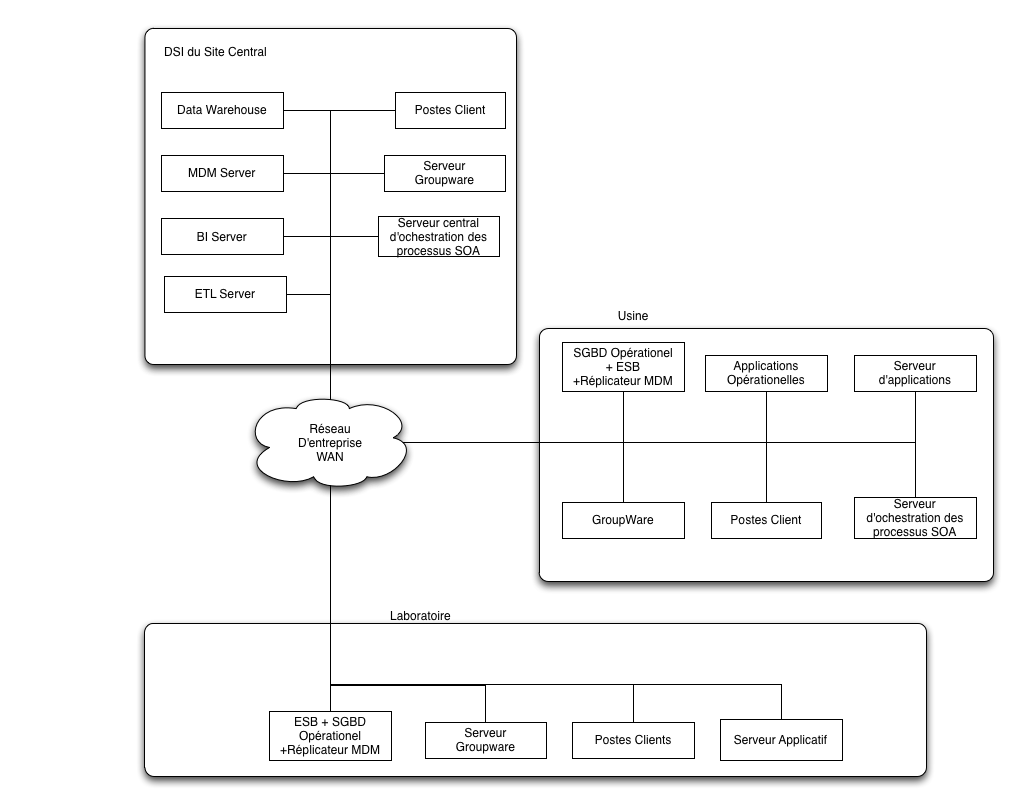
\includegraphics[scale=0.6]{DiagrameSOAPdc4.png}

\subparagraph{Infrastructure de support technique}
Afin de simplifier l'exploitation, nous proposons que l'architecture logicielle proposée soit supportée par une achitecture basée sur des machines virtuelles, limitant grandement le nombre de machines de type serveur à déployer.
Les systèmes virtuels sont facilement manipulables et peuvent être restaurés simplement en cas de défaut de machines.\\
Bien entendu les infrastructures de transport, passives et actives sont à prévoir.

\subparagraph{Architecture pour le site central}

Le site central est dans ce scenario le centre névralgique du système d'information de l'entreprise. Les services hébergés sont les suivants :\\

\begin{itemize}
\item Main dataWarehouse : Principal entrepot de données de l'entreprise, c'est lui qui constitue la base de travail pour les application de business intelligence.
\item MDM Server :  Serveur de Master data Management, en charge de la génération, du maintien, et de l'expoistion aux applications utilisatrices de la base d'exploitation de données de références.
\item BI Server : Hébergment des principaux services de business intelligence, sytème de reporting, générateurs de tableaux de bords et applicatif dédié au DataMining.
\item ETL Server : En charge de l'alimentation du dataWarehouse, assure la synchronisation des données entre les différents SGBD opérationels déployés sur les différents sites, et la synchro réciproque entre le datawarhouse et le système de master data management.
\item Serveur central d'orchestration SOA : Serveur en charge de l'orchestration des principaux processus et méta-processus de l'entreprise, il pilote les services d'orchestration déployés dans chaque site.
\item Serveur Groupware, dédié au travail collaboratif.
\end{itemize}

La totalité des postes présents sont réutilisés, moyennant éventuellement un dedéploiement de ces derniers. De plus, la création d'une DSI implique l'équipement des effectifs de ce service.

\subparagraph{Achitecture pour laboratoire & Usine}

Chaque entité de l'entreprise possède son propre SI autonome, permettant un fonctionement de l'entreprise en mode dégradé. ( Site pricipal injoignable...)
La seule différence 

\paragraph{Robustesse et tolérance aux incidents}

\subsubsection{Impact organisationnel}

\subsubsection{Plan de déploiement}

\subsubsection{Gestion du changement utilisateur}

\subsubsection{Conclusion}

\subsection{Scénario de déploiement d'un ERP}

\subsubsection{Présentation de la solution}
\paragraph{Architecture Logicielle}

\paragraph{Architecture matérielle}

\subsubsection{Ressources nécessaires}

\subsubsection{Plan de déploiement}

\subsubsection{Gestion du changement}

\subsubsection{Conclusion}